\documentclass[11pt,letterpaper]{article}
\usepackage[spanish]{babel}
%\usepackage[ansinew]{inputenc}
\usepackage[utf8]{inputenc}
%\usepackage[latin1]{inputenc}
\usepackage[letterpaper,includeheadfoot, top=0.5cm, bottom=3.0cm, right=2.0cm, left=2.0cm]{geometry}
\renewcommand{\familydefault}{\sfdefault}

\usepackage{graphicx}
\usepackage{color}
\usepackage{hyperref}
\usepackage{amssymb}
\usepackage{url}
%\usepackage{pdfpages}
\usepackage{fancyhdr}
\usepackage{hyperref}
\usepackage{subfig}

\usepackage{listings} %Codigo
\lstset{language=C, tabsize=4,framexleftmargin=5mm,breaklines=true}

\definecolor{gray}{rgb}{0.51,0.51,0.51}
\begin{document}
%\begin{sf}
% --------------- ---------PORTADA --------------------------------------------
\newpage
\pagestyle{fancy}
\fancyhf{}
%-------------------- CABECERA ---------------------
\fancyhead[L]{ 
\includegraphics[scale=0.9]{img/logo_die.pdf} }
%------------------ TÍTULO -----------------------
\vspace*{6cm}
\begin{center}
\Huge  {Metodología de Trabajo} \\
\vspace{1cm}
\huge {EL6908 - Introducción al Trabajo de Título}\\
\vspace{1cm}
\huge {\textit{Diseño e Implementación del Software de Control para el Computador a Bordo de un Pico-Satélite}}\\
%\vspace{1cm}
%\small {Título pequeño} 
\end{center}
%----------------- NOMBRES ------------------------
\vfill
\begin{flushright}
\begin{tabular}{ll}
\textbf{Autor} &: Carlos González C.\\
\textbf{Profesor Guía} &: Marcos Díaz Q.\\
\textbf{Profesor EL6908} &: Jorge Lopez H.\\
& \today\\
& Santiago, Chile.
\end{tabular}
\end{flushright}

% ·············· ENCABEZADO ············
\newpage
\pagestyle{fancy}
\fancyhf{}
%\fancyhead[L]{\rightmark}
\fancyhead[L]{\small \rm \textit{Sección \rightmark}}
\fancyhead[R]{\small \rm \textbf{\thepage}}
\fancyfoot[L]{\small \rm \textit{Estructura del capítulo 3}}
\fancyfoot[R]{\small \rm \textit{EL6908 - Introducción al Trabajo de Título}}
%\fancyfoot[C]{\thepage}
\renewcommand{\sectionmark}[1]{\markright{\thesection.\ #1}}
\renewcommand{\headrulewidth}{0.5pt}
\renewcommand{\footrulewidth}{0.5pt}

% =============== INDICE ===============

\tableofcontents
\listoffigures
% \listoftables

% =============== ANALISIS ===============
\newpage
\section{Flujo de trabajo}

A grandes rasgos se debe considerar el objetivo general del proyecto que es la ``La implementación del software de control del computador a bordo de un pico-satélite''. Esto significa a modo general seguir el diagrama de flujo de la figura \ref{flujo} donde se parte por una etapa de definición de requerimientos los cuales son luego diseñados e implementados y se considera el soporte de esta aplicación durante la vida útil del proyecto.

%···················· FIGURE ····················
\begin{figure}[!hb]
\centering

\includegraphics[width=0.8\textwidth]{img/flujo_desarrollo.jpg}
\caption{Diagrama de flujo del proyecto} \label{flujo}
\end{figure}
%················································

No obstante el flujo general esconde lo que realmente ocurre en las etapas de diseño e implementación, que son la parte gruesa del tiempo  esfuerzo dedicado a un proyecto de estas características.

\subsection{Ciclo de desarrollo}

El ciclo de desarrollo detallado de un proyecto de software como el que acá se describe cuenta de cinco etapas fundamentales (ver figura \ref{metod}):

\begin{itemize}
	\item \textbf{Análisis de requerimientos:} Se deben esclarecer y detallas los requerimientos del proyecto para una determinada etapa. El desarrollo debe estar enfocado en cumplir estos requerimientos y nada más allá.
	
	\item \textbf{Diseño:} Se diseña la solución que permite cumplir los requerimientos, es una etapa conceptual que permite definir las herramientas necesarias para su implementación.
	
	\item \textbf{Implementación:} Se implementa la solución diseñada utilizando las herramientas disponibles. Se concreta esta etapa del proyecto y el resultado es un prototipo funcional.
	
	\item \textbf{Pruebas:} Se genera un banco de pruebas cuyo objetivo es demostrar que la implementación cumple con los requerimientos solicitados.
	
	\item \textbf{Evolución:} A partir de las pruebas pueden sugerirse correcciones o cambios en la implementación, pero en este punto también pueden surgir nuevos requerimientos o bien comenzar una nueva iteración sobre las etapas siguientes del proyecto.
	
%···················· FIGURE ····················
\begin{figure}[!hb]
\centering
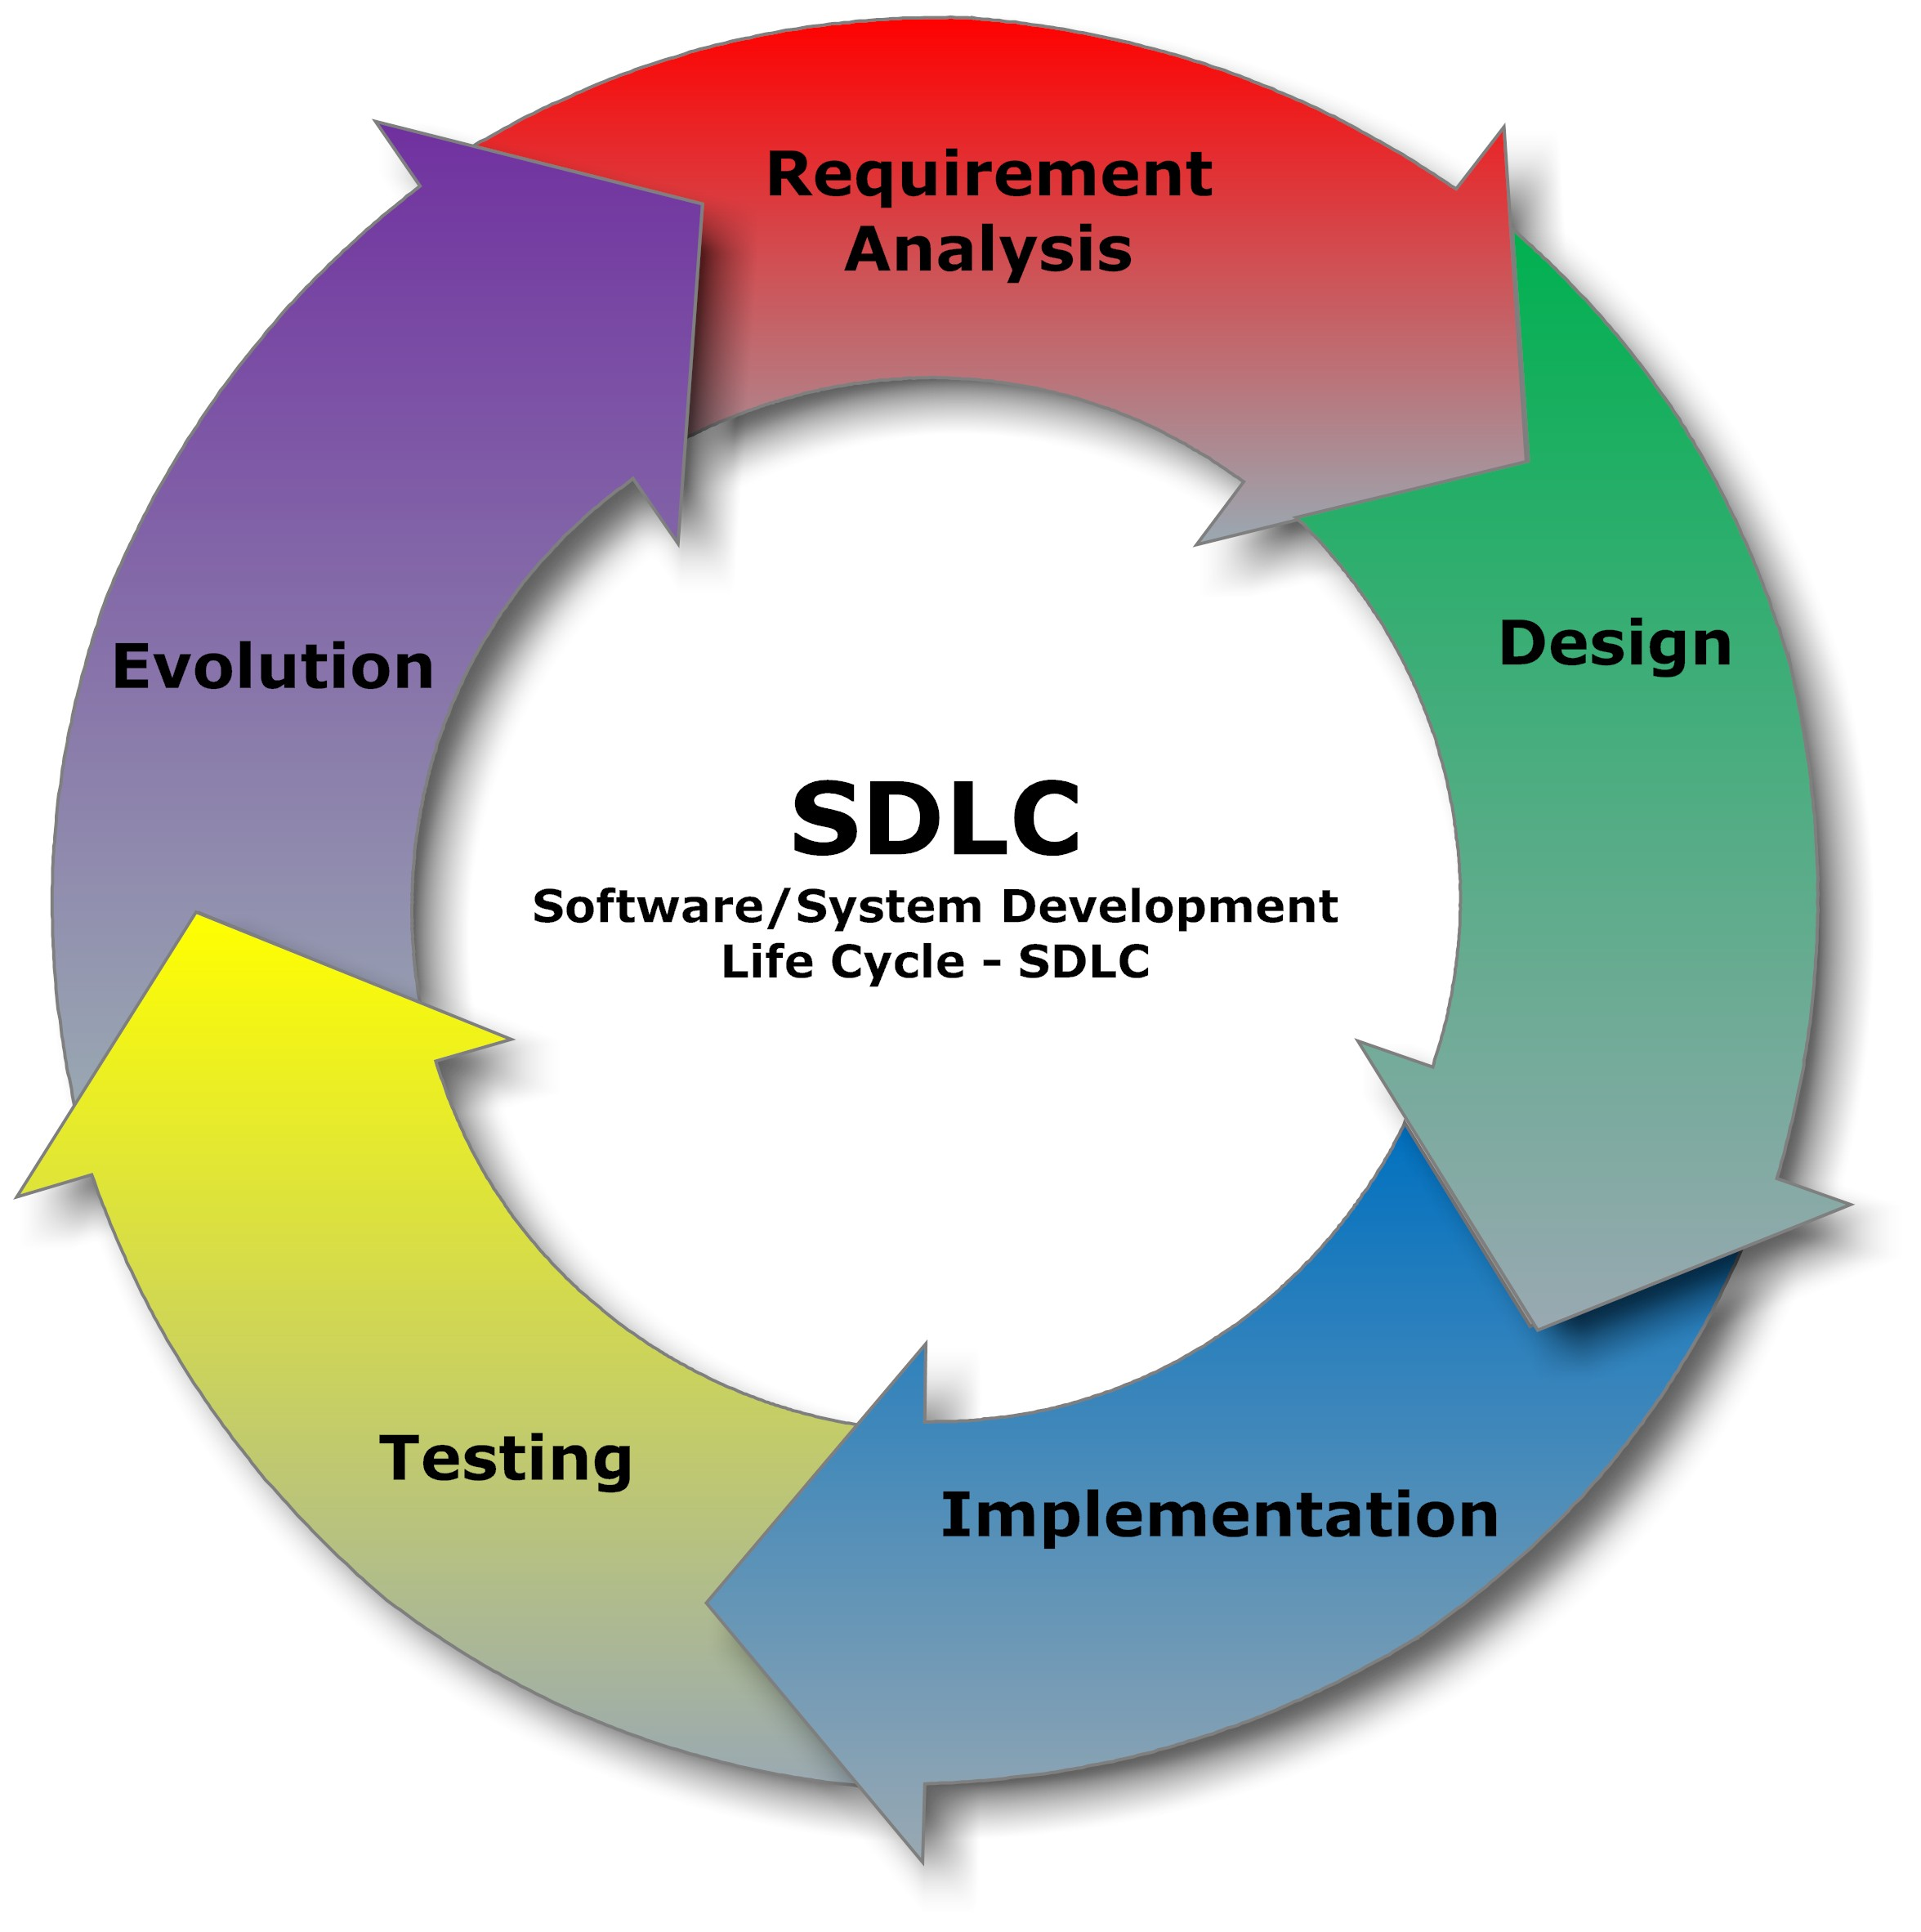
\includegraphics[scale = 0.1]{img/sdlc.jpg}
\caption{Ciclo de desarrollo de software} \label{metod}
\end{figure}
%················································

Es importante destacar que este esquema implica un ciclo de desarrollo, donde su final no siempre está claro pues los requerimientos evolucionan con el tiempo o bien sugiere un método de trabajo iterativo.
	
\end{itemize}

\newpage
\section{Metodología}

Considerando el flujo de desarrollo típico de un proyecto de estas características la metodología de trabajo acordada para este proyecto se sustenta en los siguientes puntos:

\begin{itemize}
	\item Se sigue una metodología de trabajo iterativa, esto es en cada etapa se fija una cantidad limitada de requerimientos que son desarrollados y probados. Una vez que se termina una iteración, se producen mejoras o aumento de requerimientos sobre la base desarrollada anteriormente.
	
	\item Las decisiones de diseño  requerimientos se van tomando de manera incremental, al comienzo de cada iteración y son evaluadas al final de cada ciclo.
	
	\item Todo con el objetivo de contar siempre con una versión funcional del software de control, aunque en las primeras etapas sólo cumpla una cantidad limitadas de requerimientos.
	
	\item Al ser un proyecto aeroespacial, es una misión crítica, por lo cual todas las decisiones de diseño e implementación deben ser tomadas considerando la forma más simple y clara posible. Esto para facilitar la detección y limitar el origen de los errores.
	
\end{itemize}


% % ============= BIBLIOGRAFIA ==============
% \newpage
% \begin{thebibliography}{5}
% 	\bibitem{cmos} R. Jacob Baker, \textit{CMOS. Circuit Design, Layout, and Simulation}, 2nd ed., USA: IEEE Press, 2005
% 	
% \end{thebibliography}

\end{document}

% % ················ IMAGEN ·················
% \begin{figure}[ht!]
% \centering
% \fbox{\includegraphics[scale=0.6]{img/flujo.png}}
% \caption{Flujo de caja anual}\label{flujo}
% \end{figure}
% %··········································

% % ················ IMAGEN ·················
% \begin{figure}[ht!] \centering
% \subfloat[Esquemático]{\includegraphics[scale=0.44]{img/seguidor.png}}
% \subfloat[Simulación]{\includegraphics[scale=0.45]{img/seguidor1.png}}
% \caption{Simulación como seguidor de voltaje}\label{seguidor}
% \end{figure}
% %··········································